\documentclass[border=6pt]{standalone}
\usepackage{tikz}
\usetikzlibrary{arrows.meta,positioning,calc,shapes.geometric,fit,backgrounds,patterns,matrix,decorations.pathreplacing}
\begin{document}
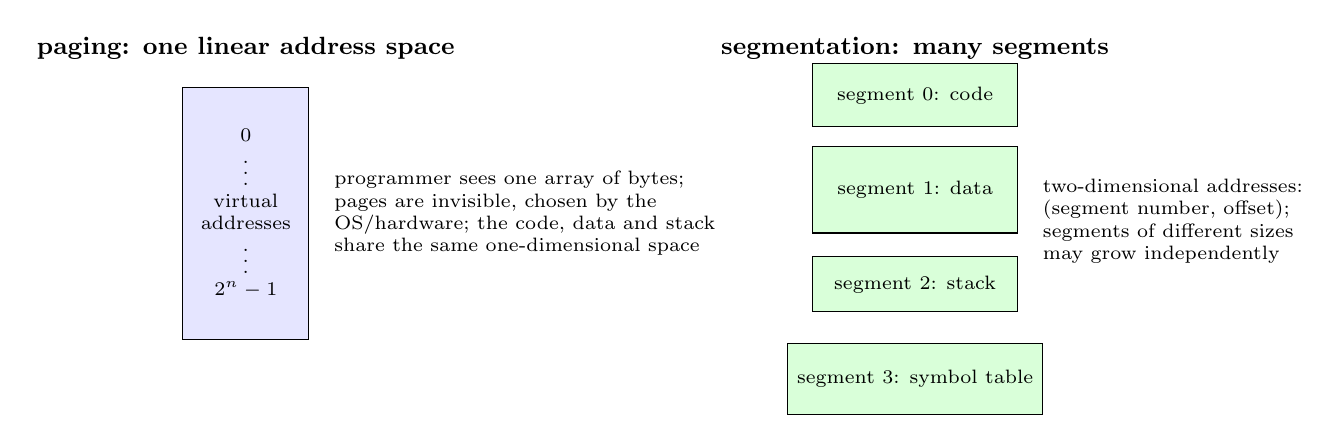
\begin{tikzpicture}[>=Stealth,font=\small]
\tikzstyle{b}=[draw,font=\scriptsize,align=center]
\node[font=\small\bfseries] at (2,3.2) {paging: one linear address space};
\node[b,minimum width=1.6cm,minimum height=3.2cm,fill=blue!10] at (2,1.1) {0\\ \vdots\\ virtual\\ addresses\\ \vdots\\ $2^n-1$};
\node[font=\scriptsize,align=left,anchor=west] at (3.0,1.1) {programmer sees one array of bytes;\\ pages are invisible, chosen by the\\ OS/hardware; the code, data and stack\\ share the same one-dimensional space};
\node[font=\small\bfseries] at (10.5,3.2) {segmentation: many segments};
\foreach \i/\t/\h in {0/{segment 0: code}/0.8,1/{segment 1: data}/1.1,2/{segment 2: stack}/0.7,3/{segment 3: symbol table}/0.9} \node[b,minimum width=2.6cm,minimum height=\h cm,fill=green!15] at (10.5,2.6-\i*1.2) {\t};
\node[font=\scriptsize,align=left,anchor=west] at (12.0,1.0) {two-dimensional addresses:\\ (segment number, offset);\\ segments of different sizes\\ may grow independently};
\end{tikzpicture}
\end{document}
